\section{Definiowanie planu w postaci mapy}
Dozwolona przestrzeń zewnętrzna poruszania się robotów zdefiniowana jest poprzez mapę reprezentowaną w postaci dwuwymiarowej tablicy, gdzie odpowiednie wartości określają ściany, poszukiwane obiekty (ranni ludzie), stany dozwolone, stany zakazane i inne. Mapy generowane są za pomocą programu \href{https://www.mapeditor.org/}{Tiled}. Interfejs programu został przedstawiony na Rys. \ref{fig:tiled}.
\begin{figure}[H]
    \centering
    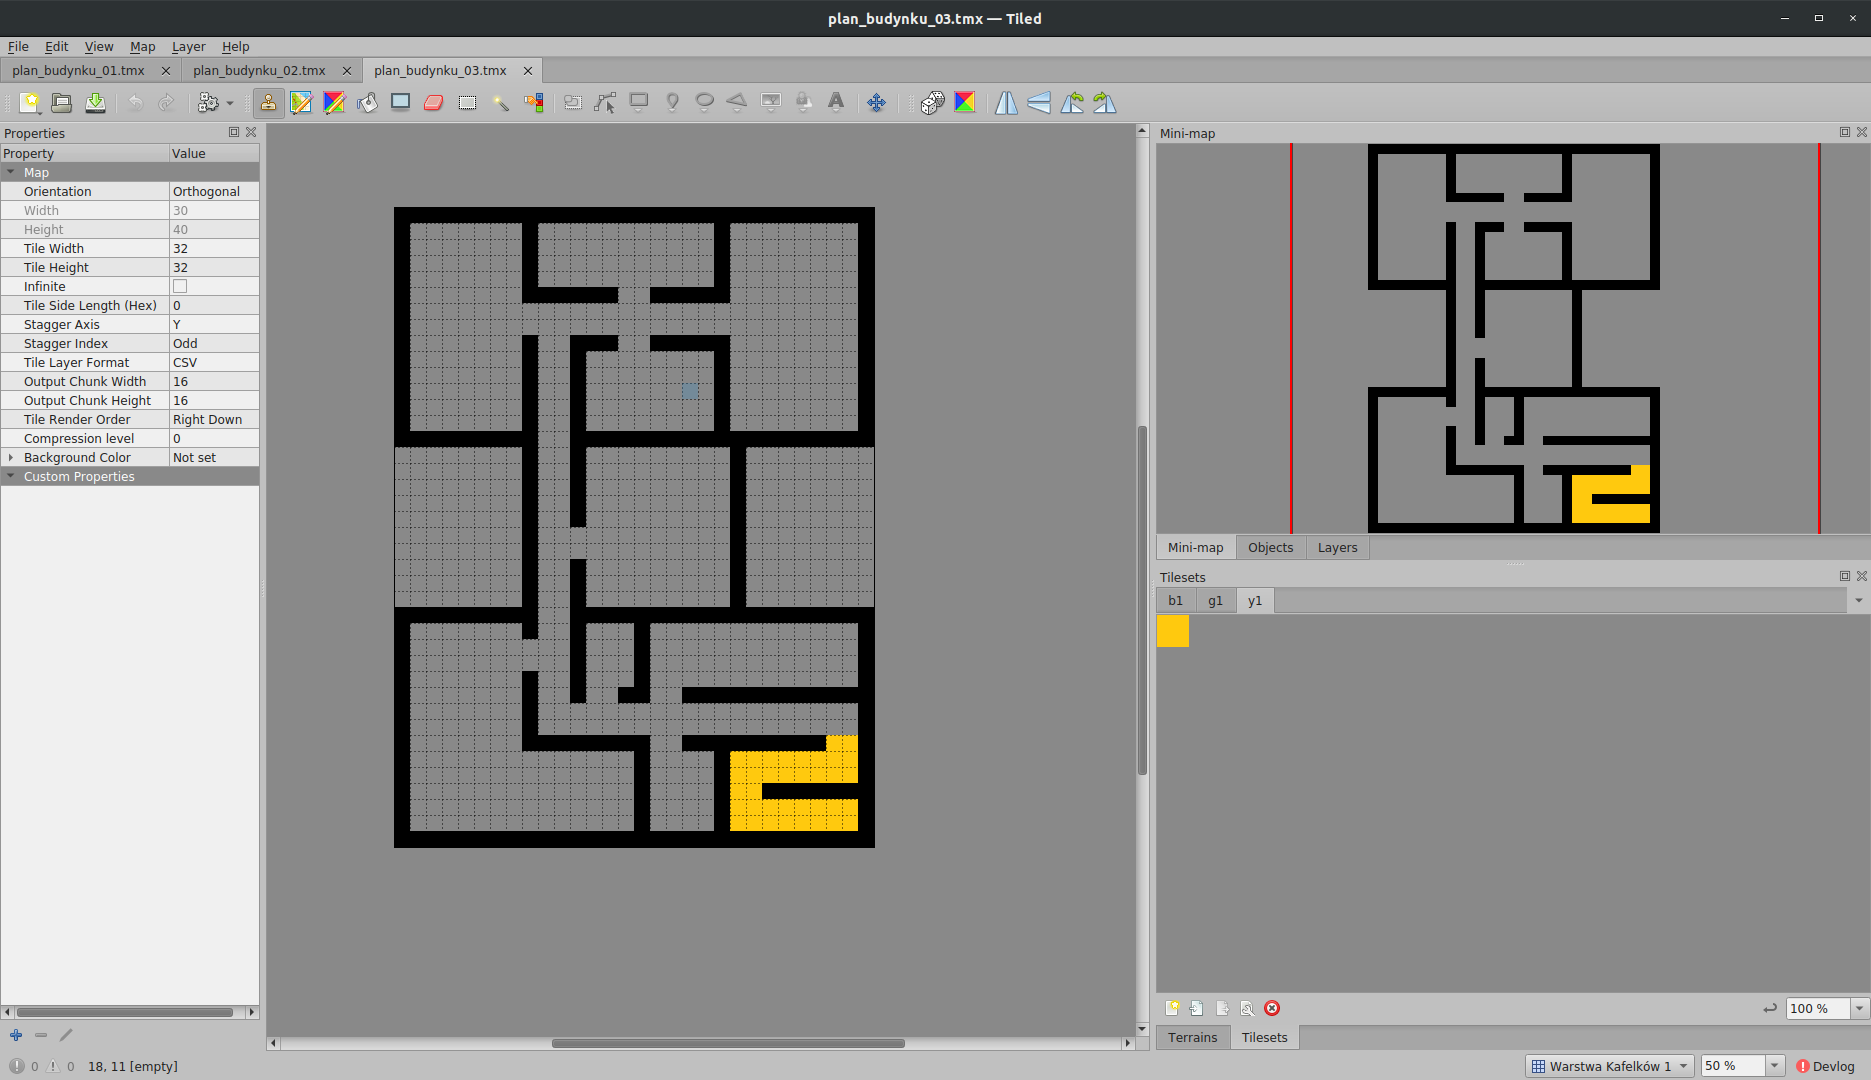
\includegraphics[width=0.7\textwidth]{figures/tiled}
    \caption{Okno edytora map 2D \textit{Tiled}}
    \label{fig:tiled}
\end{figure}

Rys. \ref{fig:mapy} przedstawia przykładowe, utworzone w celach testowych mapy.
\begin{figure}[H]
    \centering
    \begin{subfigure}[b]{0.3\textwidth}
        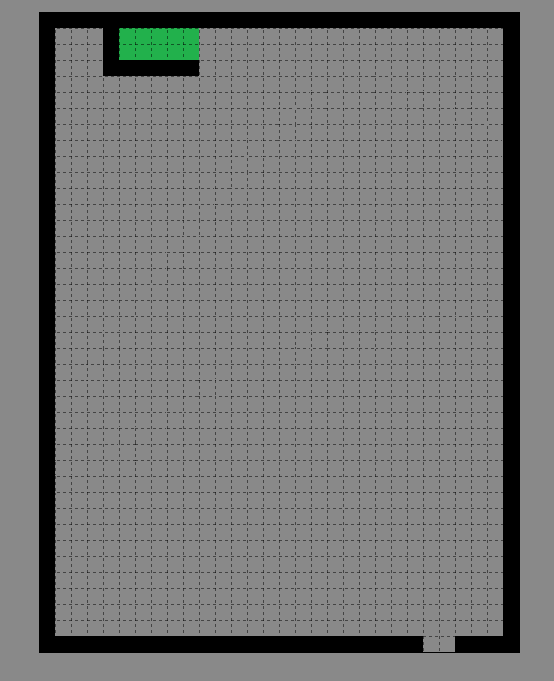
\includegraphics[width=\textwidth]{figures/p1.png}
        \caption{}
        \label{fig:gull}
    \end{subfigure}
    ~
    \begin{subfigure}[b]{0.3\textwidth}
        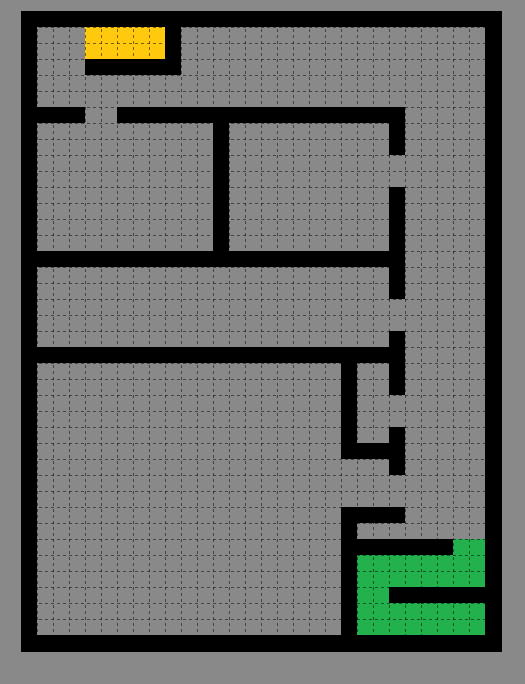
\includegraphics[width=\textwidth]{figures/p2.png}
        \caption{}
        \label{fig:tiger}
    \end{subfigure}
    ~
    \begin{subfigure}[b]{0.3\textwidth}
        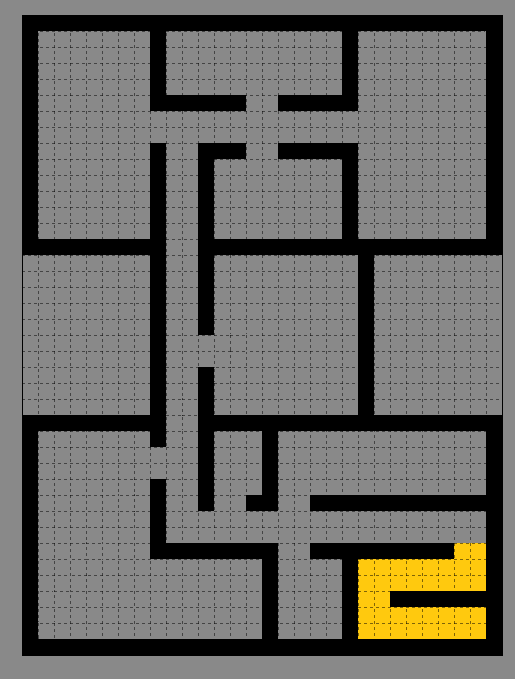
\includegraphics[width=\textwidth]{figures/p3.png}
        \caption{}
        \label{fig:mouse}
    \end{subfigure}
    \caption{Przykładowe mapy o różnym stopniu złożoności}
    \label{fig:mapy}
\end{figure}

Zielone i pomarańczowe obszary oznaczają odpowiednio schody w górę i w dół.\\
\\
Osoby poszkodowane rozmieszczane są poprzez funkcję \textit{random} w losowych miejscach. Ilość poszkodowany ustalana jest każdorazowo odgórnie do celów symulacji. Położenie oraz ilość celi nie są znane dla jednostki centralnej oraz roju robotów poszukiwawczych.\\
\\
Po przygotowaniu map są one eksportowane do pliku w formacie *.json. Plik ten zawiera wyeksportowaną mapę zapisywaną w postaci jednowymiarowej tablicy i inne dane dotyczące planu. Plik następnie jest parsowany za pomocą skryptu w celu uzyskania dwuwymiarowej reprezentacji mapy i możliwości zapisu jej w postaci tekstowej (np.\@ w celu wyświetlenia, ręcznej edycji mapy) lub w postaci binarnej. Sparsowana mapa jest plikiem wejściowym do programu. Jednostka centralna pobiera dane o ściana, dzięki czemu ma możliwość wyznaczenia celów przeszukiwania oraz wstępnych tras dla robotów.